% Tutoriales Workshop
\subsection{TRAC}

\subsubsection{Qué es Trac}
Trac es un manejador de proyectos y bugs.
Permite enlazar información entre una base de datos de errores de software, un sistema de control de versiones y el contenido de un wiki.\\
Está escrito en Python y publicado bajo la licencia BSD modificada.

\subsubsection{Características}
\begin{itemize}
    \item Administración de proyectos (Roadmap, Milestones, etc.).
    \item Sistema de tickets (bug tracking, tareas, etc.).
    \item Administración fina de permisos de acceso (desde la versión 0.11).
    \item Linea de tiempo para toda la actividad reciente.
    \item Wiki.
    \item Reporte customizado.
    \item Interfaz de web VCS.
    \item RSS Feeds.
    \item Soporte de múltiples proyectos.
    \item Aumento de funcionalidades por extensiones o plugins.
    \item Formato iCalendar.
    \item Soporte de múltiples repositorios por ambiente (desde la 0.12)
\end{itemize}


\subsubsection{Instrucciones de uso}
Crear una página wiki:
  \begin{itemize}
    \item Editamos una página y escribimos una ``WikiWord''. Al guardar la página, la WikiWord sera presentada como un link a una página nueva y, siguiendo este link, podrás pasar a editar la nueva página.
    \item Otra forma de crear una página en la wiki es accediendo a ella a
    través del navegador,por ejemplo\\
    \url{http://csrg.inf.utfsm.cl/taller_trac/wiki/newpage}\\ y presionar en
    ``Edit This page link'', o explicitando específicamente el nombre que
    quieres que tenga el link visualizado en la página wiki:
        \begin{center}\textbf{\lbrack wiki:NombreDePagina Nombre de Link\rbrack}\end{center}
    \item Para evitar que Trac reconozca una WikiWord, se le antepone ! a la palabra.
  \end{itemize}


\subsubsection{Ejercicio}
\begin{description}
  \item[Creación de las Fichas de usuarios]:
  \begin{itemize}
    \item Creamos una página con la información personal de uno:\\
    \url{http://csrg.inf.utfsm.cl/taller_trac/wiki/NombreApellido/}
    \item Dentro de ella, llenamos nuestros datos utilizando la siguiente
    plantilla:\\
\begin{verbatim}
== Nombre Apellido ==

|| '''Nombre:''' || Nombre Apellido ||
||'''Foto:'''|| [[Image(nombreimagen.png)]] ||
|| '''Cumpleaños:''' || fecha de tu cumpleaños ||
|| '''Celular:''' ||  ||
|| '''Telefono:''' ||  ||
||'''MSN:'''|| ||
||'''SkypeID:'''||  ||
||'''YahooID:'''||  ||
||'''Dirección:'''|| ||
||'''GMail:'''|| ||
|| '''Mail:''' ||  ||
\end{verbatim}
    \item Crear un link a su página creada dentro de la página principal, de
    la siguiente forma:
        \begin{center}\textbf{\ \ \ *\ \lbrack wiki:NombreApellido Nombre Apellido\rbrack}\end{center}

  \end{itemize}

\item[Asignación de tareas]:
\begin{enumerate}
    \item Cree 2 tareas cualquiera y asigne las a alguno de sus compañeros
    (anotando el usuario de los responsables, separados por comas).
    \item Pruebe diferentes atributos que puede asignarle a una tarea.
\end{enumerate}

\end{description}

\newpage
%%%%%%%%%%%%%%%%%%%%%%%%%%%%%%%%%%%%%%%%%%%%%%%%

\subsection{Git}

\subsubsection{Qué es GIT}

GIT es un software de control de versiones (SCM) open source, diseñado por Linus Torvalds para ser utilizado de manera distribuida. Al ser descentralizado, posee
la gran ventaja de poder trabajar sobre copias locales sin depender de un nodo central.

\subsubsection{Instrucciones de uso}

Existen una serie de comandos que son los más utilizados para trabajar con git, sin embargo por el tiempo solo se verán los que utilizaremos en el tutorial.

\begin{itemize}
    \item git init: Permite iniciar un repositorio git. No será utilizado en este tutorial.
    \item git clone $<$repositorio$>$: Permite crear una copia local de un repositorio remoto.
    \item git add $<$archivo$>$: Permite agregar bajo el control de git a un archivo.
    \item git commit -sm 'Mensaje': Permite comprometer un cambio en el repositorio.
    \item git pull: Obtiene cambios remotos en la copia local.
    \item git push: Envía cambios locales a repositorio remoto.
\end{itemize}


\subsubsection{Ejercicio}

\textbf{Objetivo}

 En 3 equipos, se realizará un pequeño programa en lenguaje ANSI C de manera colaborativa. La estructura del código será:

\begin{itemize}
    \item ssg.c: Archivo principal, debe llamar a la función plot
    \item plot.c: Definición de función plot, debe mostrar un mensaje del tipo: ``Plotting data...''. Incluye a su declaración (.h)
    \item plot.h: Declaración del prototipo de la función plot
    \item Makefile: Archivo makefile
\end{itemize}

\textbf{Desarrollo}

\begin{enumerate}

    \item Clonar repositorio git (git clone)
    \item Desarrollo de código (disponible en la siguiente sección)

        \begin{itemize}
            \item Equipo 1: Desarrollo de ssg.c
            \item Equipo 2: Desarrollo de plot.c y plot.h
            \item Equipo 3: Desarrollo de Makefile
        \end{itemize}

    \item Agregar archivos bajo el control de git (git add)
    \item Comprometer cambios locales (git commit)
    \item Comprobar cambios globales (git pull)
    \item Enviar cambios locales a rama principal (git push)

\end{enumerate}

\textbf{Código fuente}

\begin{itemize}
	\item \texttt{ssg.c}
		\verbatiminput{../3-workshop/2-tutoriales/src/git/ssg.c}

	\item \texttt{plot.c}
		\verbatiminput{../3-workshop/2-tutoriales/src/git/plot.c}

	\item \texttt{plot.h}
		\verbatiminput{../3-workshop/2-tutoriales/src/git/plot.h}

	\item \texttt{Makefile}
		\verbatiminput{../3-workshop/2-tutoriales/src/git/Makefile}
\end{itemize}

\newpage
%%%%%%%%%%%%%%%%%%%%%%%%%%%%%%%%%%%%%%%%%%

\subsection{\LaTeX}


\subsubsection{Qué es Latex}
Sistema de composición de textos, orientado especialmente a la
creación de libros, documentos científicos y técnicos que contengan
fórmulas matemáticas.

\subsubsection{Instrucciones de uso}

Para ésta herramienta sólo nos limitaremos a utilizar un archivo \textbf{tex},
y un comando para compilarlo a \textbf{pdf}.
Si nuestro archivo fuera \texttt{ejemplo.tex}, el procedimiento sería:
\begin{verbatim}
    $ pdflatex ejemplo.tex
\end{verbatim}
Donde finalmente podremos obtener un archivo \texttt{ejemplo.pdf}

Explicación comandos dentro del documento:
\begin{itemize}
    \item \texttt{$\backslash$documentclass}: Declaración del documento.
    \item \texttt{$\backslash$usepackage}: Uso de un paquete determinado (como un import, include, etc)
    \item \texttt{$\backslash$title}: Declaración del título del documento.
    \item \texttt{$\backslash$author}: Declaración de el o los autores.
    \item \texttt{$\backslash$section}: Declaración de una nueva sección del documento.
    \item \texttt{$\backslash$subsection}: Declaración de una nueva subsección del documento.
\end{itemize}

\subsubsection{Ejercicio}
Generar un informe~\footnote{Archivo principal \texttt{informe.tex}} que contenga:

\begin{itemize}
    \item Descripción Proyecto. (\texttt{src/descripcion.tex})
    \item Requerimientos. (\texttt{src/requerimientos.tex})
    \item Información de cada desarrollador. (\texttt{src/informacion.tex})
\end{itemize}

\newpage
%%%%%%%%%%%%%%%%%%%%%%%%%%%%%%%%%%%%%%%%%%

\subsection{Planner}

\subsubsection{Qué es Planner}
Planner es una herramienta para planear, programar y seguir proyectos para el
escritorio GNOME. Es una aplicación GTK+ escrita en C y licenciada bajo GPL
(versión 2 o posterior).

\subsubsection{Características}
Puede almacenar sus datos en ficheros XML o en una base de datos
postgresql. Los proyectos pueden ser impresos en PDF o exportados a HTML para
una visualización simple desde cualquier navegador web.

El programa permite:
\begin{itemize}
    \item Gestión de calendarios
    \item Gestión de recursos
    \item Seguimiento del avance del proyecto
    \item Enlazar tareas
    \item Exportación a diferentes formatos
\end{itemize}

\begin{center}
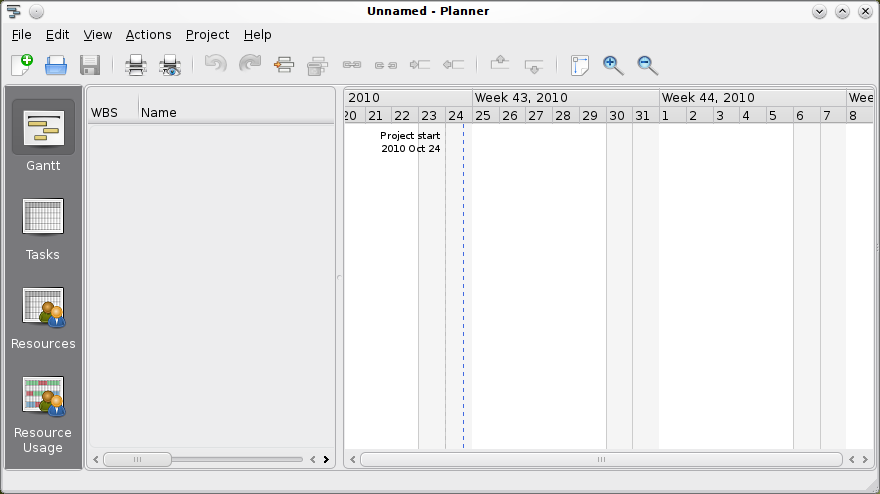
\includegraphics[scale=0.6]{../3-workshop/2-tutoriales/img/planner_1}
\end{center}

\subsubsection{Instrucciones de uso}
\begin{description}
    \item[Agregar recursos]:
\begin{enumerate}
    \item Click en Resources.
    \item Click derecho y click en "Insert Resource".
    \item Click derecho y click en "Editar Resource".
    \begin{enumerate}
        \item Poner nombre, nombre corto, tipo y costo según sea el caso.
    \end{enumerate}
\end{enumerate}

    \item[Creación de una tarea]:
\begin{enumerate}
    \item Click derecho y click en "Insert Task"
    \item Doble click en la tarea nueva para abrir su edición.
    \begin{enumerate}
        \item Poner nombre, duración.
        \item Asignar recursos.
        \item Indicar predecesores si es ese el caso.
    \end{enumerate}
\end{enumerate}

    \item[Generar pdf]:
\begin{enumerate}
    \item Ir a "File"
    \item Ir a "Print..."
    \item Seleccionar "Output Format: pdf"
    \item Ponerle un nombre al archivo y elegir donde será guardado.
    \item Click en "Print".
\end{enumerate}


\item[Recuerda al final guardar el proyecto.]

\end{description}

\subsubsection{Ejercicio}
Tomando en consideración los requerimientos de la herramienta, realice una
aproximación de la carta gantt asignando tiempos y recursos correspondientes.
En los recursos, agregue a los miembros de su grupo, y planee la actividad
para el primer mes de trabajo.

\newpage
%%%%%%%%%%%%%%%%%%%%%%%%%%%%%%%%%%%%%%%%%%

\subsection{Skype}

\subsubsection{Qué es Skype}

Skype es un software para realizar llamadas sobre Internet (VoIP). Permite comunicación entre computadores y teléfonos fijos, mediante el uso de créditos. También soporta comunicación mediante video y conferencias entre varias personas.

\subsubsection{Instrucciones de uso}

\textbf{Preliminares}

\begin{itemize}
    \item Descargar cliente Skype
    \item Crear cuenta Skype
    \item Agregar contactos
\end{itemize}

\textbf{Conferencias}

Debido a que las conferencias se realizan entre varias personas en un mismo lugar, se hace indispensable la utilización de dispositivos que faciliten dicha tarea, por lo que
contar con un hardware especializado para ello, permite establecer comunicaciones acorde a lo planeado.

Para dicho propósito usualmente se utiliza un dispositivo denominado Voice Station, el cual realiza la tarea de reproducir sonido e interpretarlo (micrófono), además de permitir marcado telefónico, por lo que mediante una pequeña configuración con un computador, más el agregado de poseer una cuenta Skype para marcado internacional, puede reemplazar perfectamente el uso de un teléfono común y corriente.

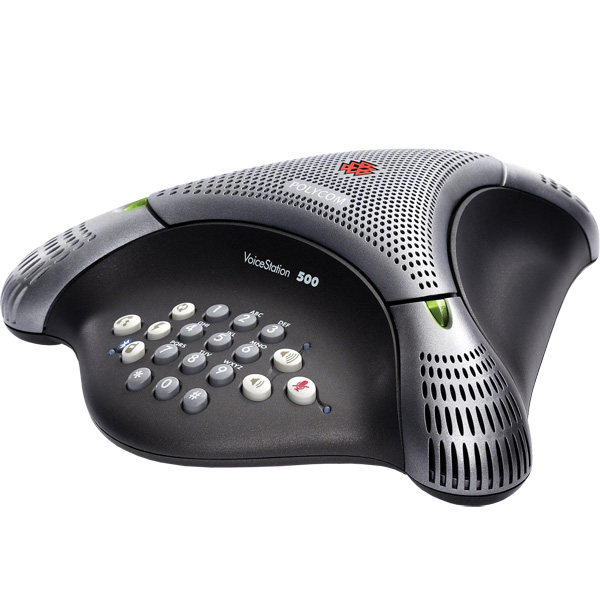
\includegraphics[scale=0.4]{../3-workshop/2-tutoriales/img/voicestation}

\subsubsection{Ejercicio}

Por último, intentaremos establecer una conferencia mediante la utilización de audio, entre 2 o más participantes.

\begin{enumerate}
    \item Abrir cliente Skype
    \item Crear cuenta de usuario
    \item Agregar a otros usarios
    \item Establecer una pequeña conferencia (audio)
\end{enumerate}


